\begin{figure}
    \begin{center}
    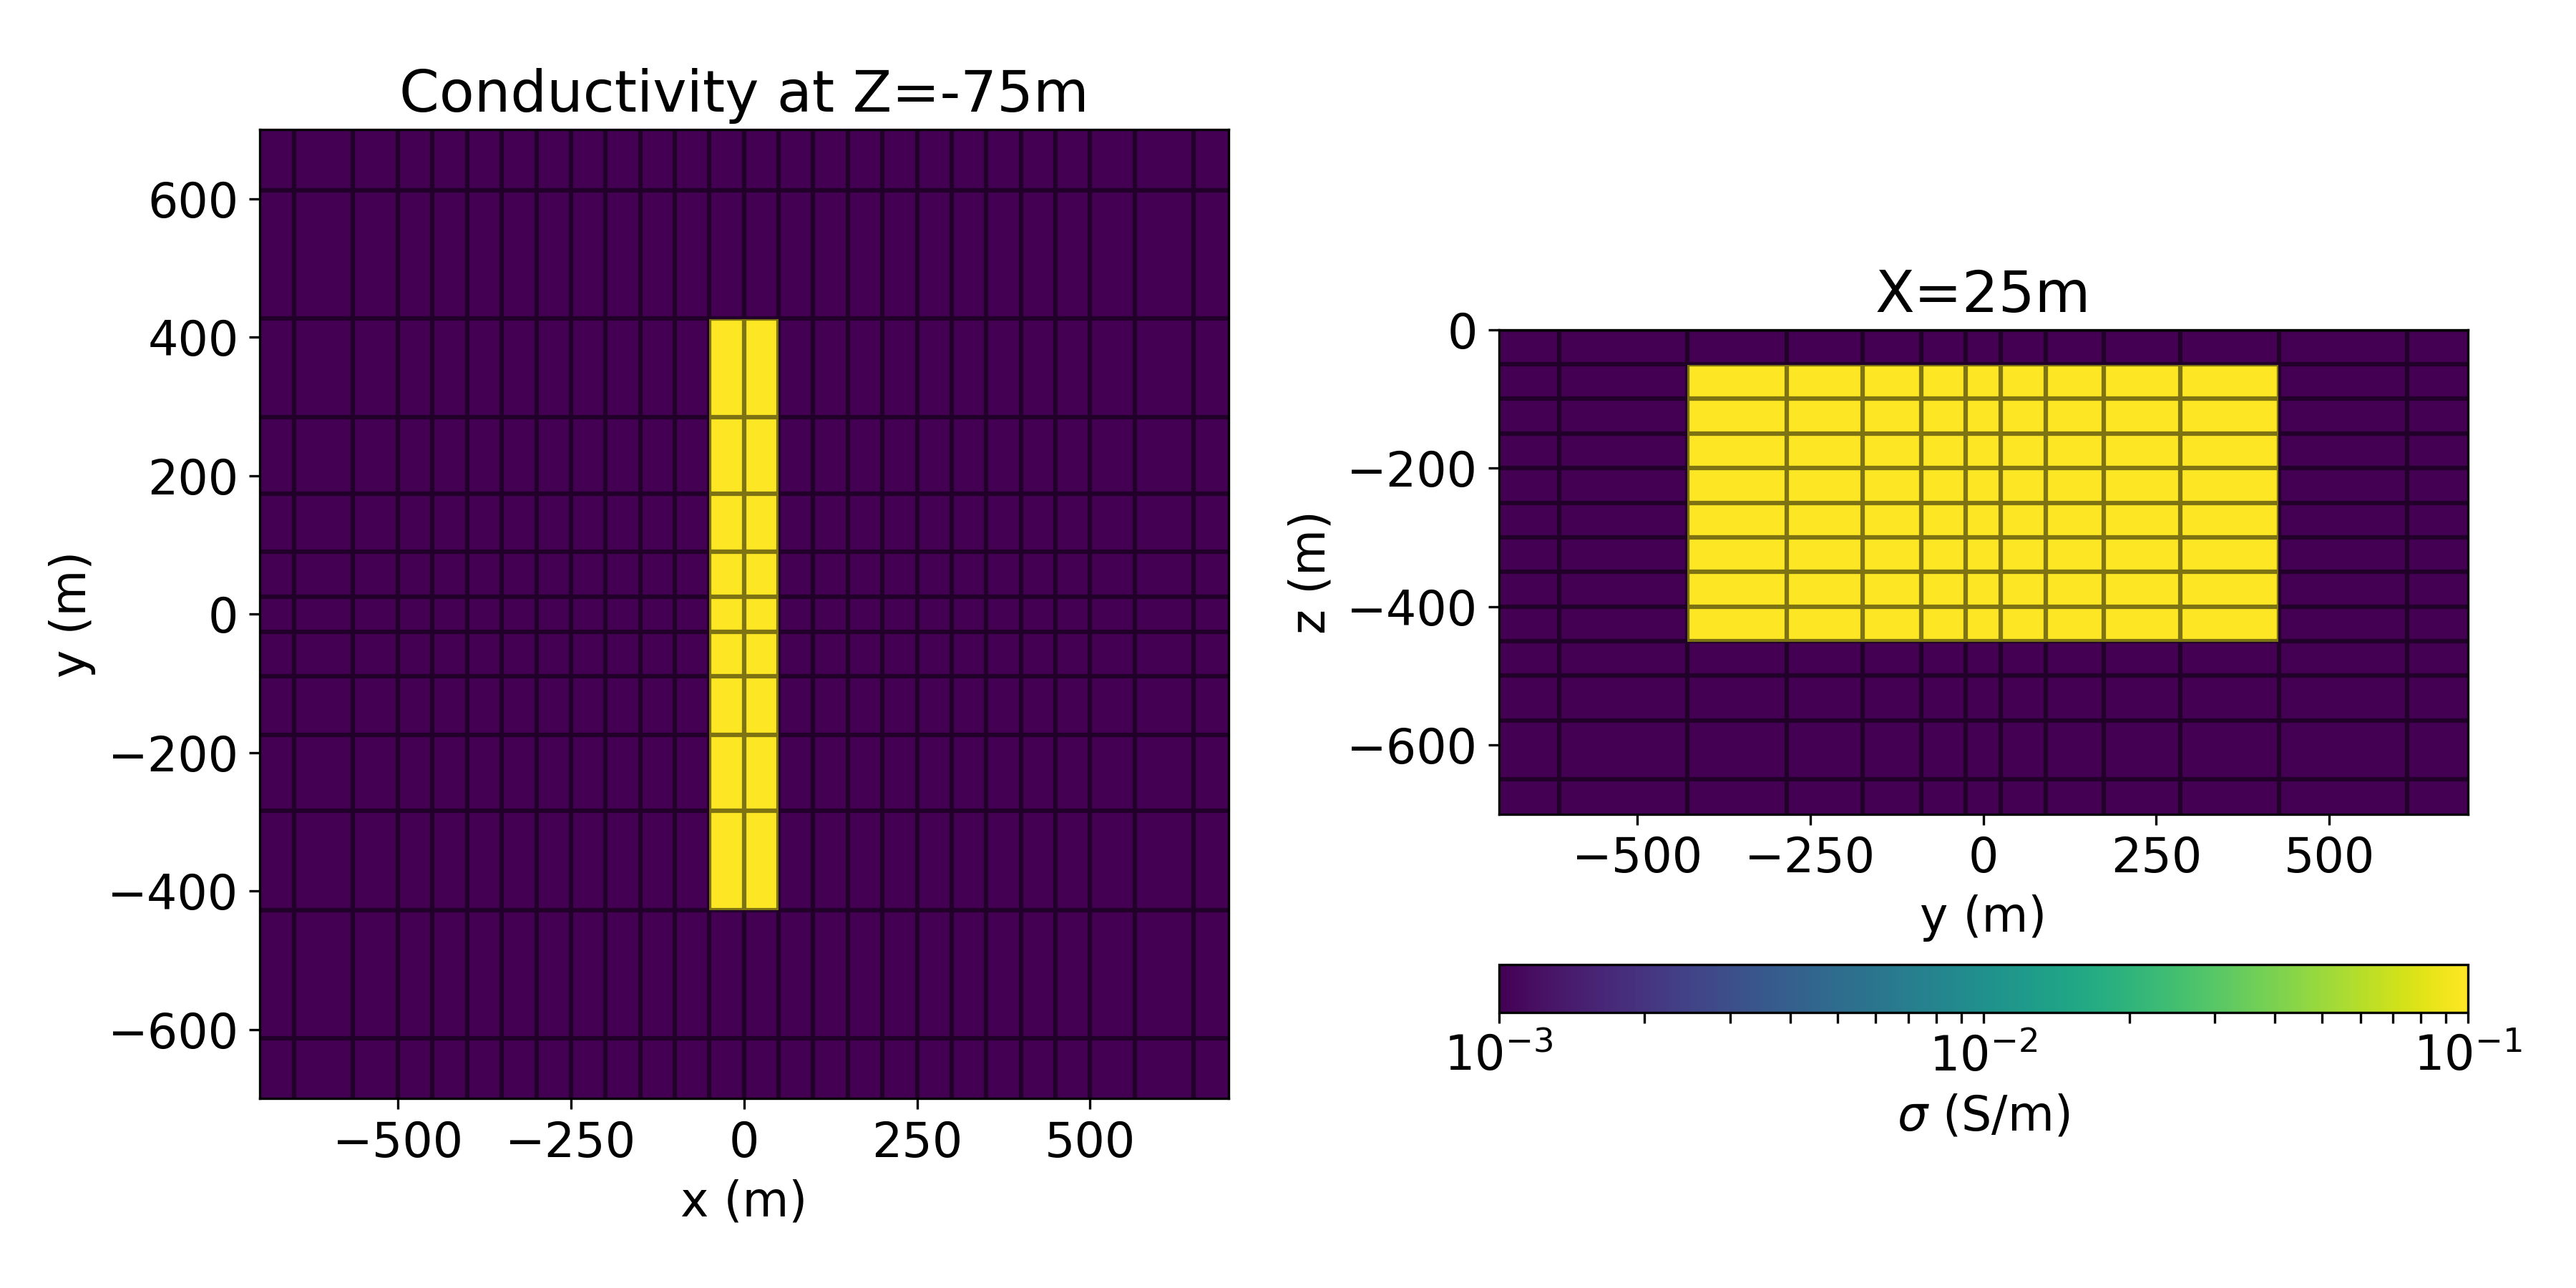
\includegraphics[width=0.8\columnwidth]{figures/plate-model.png}
    \end{center}
\caption{
    Depth slice (left) and cross section (right) through the model of a conductive plate (10 $\Omega$m) in a resistive half-space (1000 $\Omega$m).
    The mesh extends sufficiently far according to the diffusion distance for the time domain EM problem (see for example https://em.geosci.xyz).
}
\label{fig:plate-model}
\end{figure}

